\documentclass{article}
\usepackage{setspace}
\usepackage{float}
\doublespacing

\usepackage{arxiv}
\usepackage[utf8]{inputenc} % allow utf-8 input
\usepackage[T1]{fontenc}    % use 8-bit T1 fonts
\usepackage{hyperref}       % hyperlinks
\usepackage{url}            % simple URL typesetting
\usepackage{booktabs}       % professional-quality tables
\usepackage{amsfonts}       % blackboard math symbols
\usepackage{nicefrac}       % compact symbols for 1/2, etc.
\usepackage{microtype}      % microtypography
\usepackage{graphicx}
\usepackage{natbib}
\usepackage{doi}

\title{Parallel Matrix Computations in Quantitative Finance}

%\date{November 16, 2025}	% Here you can change the date presented in the paper title

\author{ 
	\href{https://orcid.org/0000-0000-0000-0000}
	{
		
\includegraphics[scale=0.06]{orcid.pdf}
		\hspace{1mm}Abigail M. ~Johnson}
		\thanks{https://github.com/magescher/ParallelComputing} \\
	    Chandra Department of Electrical and Computer Engineering \\
	    The University of Texas at Austin\\
	    Austin, TX 78712 \\
	    \texttt{abigailjohnson@utexas.edu} \\
    }

\renewcommand{\headeright}{Technical Report}
\renewcommand{\undertitle}{Technical Report}
\renewcommand{\shorttitle}{Parallel Matrix Computations in Quantitative Finance}

%%% Add PDF metadata to help others organize their library
%%% Once the PDF is generated, you can check the metadata with
%%% $ pdfinfo template.pdf
\hypersetup{
pdftitle={Parallel Matrix Computations in Quantitative Finance},
pdfsubject={q-bio.NC, q-bio.QM},
pdfauthor={Abigail M.~Johnson},
pdfkeywords={Parallel Computing, Matrix Operations, Quantitative Finance, Performance, Benchmark},
}

\raggedbottom
\begin{document}
\maketitle

\begin{abstract}
This paper explores fine, coarse, and hybrid forms of parallelism in matrix computation workloads common in the quantitative finance industry. By evaluating various parallelism strategies, we observe where concurrency delivers real gains and where contention starts to erode. The benchmark suite is implemented in Python3 and leverages SciPy to make use of the underlying BLAS kernel. The high-level design of the benchmark suite consists of two workload modules, a command line interface to control them, and a bash script to configure and execute a series of variable performance tests. Workloads leveraging fine grained parallelism saturate quickly while coarse grained workloads continue to scale with additional CPU cores. The results underpin patterns observed in industry, where the biggest performance gains are made by tuning concurrency to workload structure and available hardware.
\end{abstract}

% keywords can be removed
\keywords{Parallel Computing \and Matrix Operations \and Quantitative Finance
    \and Performance \and Benchmark}

\section{Introduction}
This paper explores fine, coarse, and hybrid forms of parallelism in linear algebra workflows common in the quantitative finance industry. Matrix operations are a well-studied and highly optimized area, so instead of trying to outperform existing libraries, I focus on how they are employed and scaled in real-life applications. In practice, there are many quantitative finance applications that reduce to: 1) applying a single linear transformation $A$ to multiple scenario vectors $S$ and 2) solving a collection of independent linear systems. By evaluating variable parallelism strategies within these workload types, we observe where concurrency delivers real gains and where contention starts to erode, and the practical tradeoffs therein.

\section{Approach and Methodology}
\label{sec:headings}
In the design of the benchmark suite, I followed an ethos of simulating real life applications, while using abstraction and simplification where it was reasonable and practical to do so. I designed and implemented two modules to benchmark the effects of variable parallelism strategies in linear algebra workflows commonly employed in quantitative finance: applying linear transformations and solving linear systems. 

\subsection{Design}
The high-level design of the benchmark suite consists of two workload modules, a command line interface to control them, and a bash script to configure and execute a series of variable performance tests. The first module, $sameA$, benchmarks fine grained parallelism in applying a single linear transformation to multiple scenario vectors $S$; this emulates workloads such as Greek calculation and portfolio risk attribution \cite{1}. The second module, $manyA$, benchmarks coarse grained (task-level) parallelism in solving a collection of independent linear systems; this emulates many-market scenarios such as Monte Carlo engines \cite{1}. To configure and instantiate both individual workloads and the larger benchmark suite, I opted for a command line interface. This allowed for ease of implementation while promoting flexibility and future extensibility. 


\subsection{Implementation}
The benchmark suite is implemented in Python3 and leverages SciPy to make use of the underlying BLAS kernel for matrix operations. I opted for Python to focus on workload emulation instead of low-level or algorithmic optimizations via Cuda or OpenMP. This was a notable tradeoff, but a deliberate choice, as the chosen stack better emulates the development environment of a typical quantitative researcher. As noted by a finance professional at Quantos Asset Management, "Python has become the lingua franca of quantitative trading" \cite{2}. 


Both modules, $sameA$ and $manyA$, leverage the $spd$ helper to construct random symmetric positive definite (SPD) matrices of size $n$ x $n$ using the formula  $ A = X^{T} X + \lambda I$. The $sameA$ module constructs a single SPD matrix $A$, factorizes it once, and solves $A x_s = b_s$ for $S$ scenario vectors using $inner$ BLAS kernel threads. The $manyA$ module constructs and factorizes $A_s$ SPD matrices and solves  $A_s x_s = b$ where $b$ is a vector of ones. Parallelism in $manyA$ comes from using $ProcessPoolExecutor$ to distribute tasks across $outer$ worker processes and assigning $inner$ per process BLAS kernel threads. Having both $inner$ and $outer$ configurable parameters enables the $manyA$ module to express both coarse and hybrid parallelism. 

\section{Results}
\label{sec:headings}
Table 1 below details the results of running the benchmark suite configured for $256 x 256$ matrix ($n=256$) and 256 scenarios ($S=256$) on two machines: a 2020 Apple M1 with eight CPU Cores and a 2024 Apple M4 Pro with twelve CPU Cores. As illustrated in Figure 1, performance improvements for fine grained parallelism quickly plateau, and we see near identical scaling patterns on both machines, despite core count differences. In these runs, there is a slight performance boost increasing from one to two BLAS threads, but it degrades thereafter. coarse grained parallelism scaled up to four processes on the M1, and degraded thereafter. On the M4 Pro, it scaled almost linearly up to eight. For coarse grained runs, absolute throughput roughly doubles from the M1 to the M4 Pro. Hybrid parallelism provides modest gains over coarse grained parallelism on the M1 machine, but comparatively underperforms on the M4 Pro.


\begingroup
\setlength{\aboverulesep}{0pt}
\setlength{\belowrulesep}{0pt}
\renewcommand{\arraystretch}{0.85}
\footnotesize

\begin{table}[H]
  \caption{Benchmark Performance Results}
  \label{tab:table1}
  \centering
  \begin{tabular}{lrrrrrrrrrr}
    \toprule
    Test type &
    outer & inner & $n$ & $S$ &
    \multicolumn{3}{c}{Apple M1 (8 CPU core)} &
    \multicolumn{3}{c}{Apple M4 Pro (12 CPU core)} \\
    \cmidrule(lr){6-8}\cmidrule(lr){9-11}
     & & & & &
    time [s] & throughput [S/s] & rel. &
    time [s] & throughput [S/s] & rel. \\
    \midrule
    Fine    & 1 & 1 & 256 & 256 & 0.0004 & 574688.16 & 1.00 & 0.0003 & 928660.05 & 1.00 \\
    Fine    & 1 & 2 & 256 & 256 & 0.0004 & 659297.62 & 1.15 & 0.0003 &1001956.95 & 1.08 \\
    Fine    & 1 & 4 & 256 & 256 & 0.0004 & 656199.88 & 1.14 & 0.0003 & 956859.11 & 1.03 \\
    Fine    & 1 & 8 & 256 & 256 & 0.0005 & 567680.32 & 0.99 & 0.0003 & 965429.33 & 1.04 \\
    \midrule
    Coarse  & 1 & 1 & 256 & 256 & 0.7576 &   337.93 & 1.00 & 0.3810 &   671.98 & 1.00 \\
    Coarse  & 2 & 1 & 256 & 256 & 0.6000 &   426.68 & 1.26 & 0.2783 &   919.85 & 1.37 \\
    Coarse  & 4 & 1 & 256 & 256 & 0.5647 &   453.32 & 1.34 & 0.2314 &  1106.38 & 1.65 \\
    Coarse  & 8 & 1 & 256 & 256 & 0.5913 &   432.95 & 1.28 & 0.2265 &  1130.48 & 1.68 \\
    \midrule
    Hybrid  & 2 & 2 & 256 & 256 & 0.6574 &   389.42 & 1.00 & 0.2788 &   918.33 & 1.00 \\
    Hybrid  & 2 & 4 & 256 & 256 & 0.6200 &   412.93 & 1.06 & 0.2794 &   916.15 & 1.00 \\
    Hybrid  & 4 & 2 & 256 & 256 & 0.5076 &   504.31 & 1.30 & 0.2305 &  1110.56 & 1.21 \\
    \bottomrule
  \end{tabular}
\end{table}

\begin{figure}[H]  
  \centering
  \label{fig:figure1}
  \caption{Relative speedup of coarse and fine grained parallelism}
  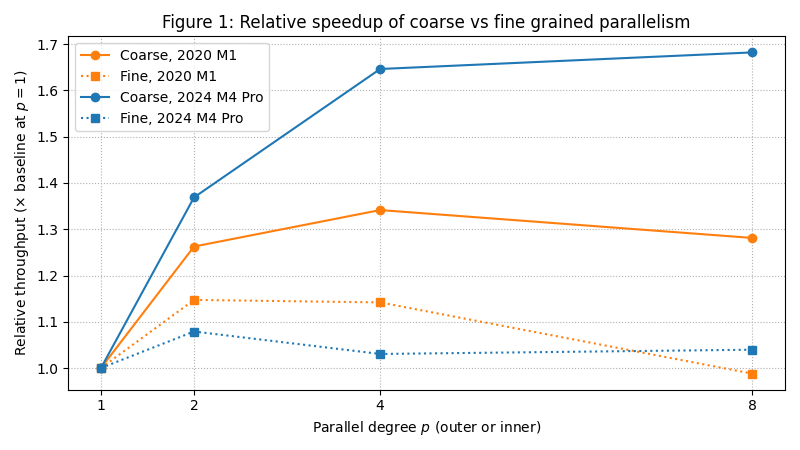
\includegraphics[width=.8\textwidth]{./benchmark_speedup_relative.png}
   %%% \caption{Relative speedup of coarse (\texttt{manyA}) and fine
  %%% (\texttt{sameA}) workloads on a 2020 Apple M1 (8-core) and a 2024 Apple M4 Pro
  %%% (12-core). Throughput for each curve is normalized to the $p=1$ configuration.}
\end{figure}

\endgroup


\section{Discussion}
\label{sec:headings}
The results underpin patterns observed in industry, where the biggest performance gains are made by tuning concurrency to both workload structure and available hardware. The results of the fine grained benchmarks are unsurprising and highlight that after initial factorization, the remaining computation is dominated by memory-bound tasks rather than CPU-bound tasks. This demonstrates that the BLAS kernel is almost entirely bandwidth limited, and additional threads only create more contention. The results of the coarse grained benchmarks are more pronounced. On both machines, task level parallelism scale well with core count. This is especially pronounced on the M4 Pro machine, and highlights architecture improvements introduced in the generation such as improved CPU cores, machine learning accelerators, and increased memory bandwidth \cite{3}. The results from the hybrid benchmarks are more nuanced and appear to highlight architectural differences such as where memory pressure first becomes limiting. Further investigation and profiling is needed to better understand the hybrid case.  


\section{Conclusions and Future Work}
\label{sec:headings}
Overall, the project and benchmark suite was successfully scoped, designed, and implemented to address the original problem statement: evaluating the effects of varying parallelism strategies in matrix computation workloads commonly employed in the quantitative finance industry. The high-level design of the benchmark suite consists of two performance test modules, a command line interface to control them, and a bash script to configure and execute a series of variable performance tests. Running the benchmark suite on two machines, a 2020 Apple M1 with eight CPU cores and a 2024 Apple M4 Pro with twelve CPU cores, demonstrate that workloads leveraging fine grained parallelism saturate quickly, while coarse grained workloads continue to scale with additional CPU cores. The results underpin patterns observed in industry where the biggest performance gains are made by tuning concurrency to workload structure and available hardware. While time did not permit their inclusion in the initial scope of this project, in the future, there are a number of topics I would like to explore further: comparing the benchmark with the Rust implemented equivalent, latest Python3 release equivalent (currently unstable), optimization with Cython, modeling popular workloads in the QuantLib library \cite{4}, and further investigation into the nuance of the hybrid case. 

\clearpage           % <-- puts References on a new page
\begingroup
\raggedright         % <-- stops ugly stretched justification
\bibliographystyle{IEEEtran}  % or another style if your class requires it
\bibliography{references}     % name of your .bib file (without .bib)
\endgroup

\end{document}

